The previous lab assignments have been primarily focused on practical applications. CRC Calculations, PWM Modulation, and Stop Watch functionality. But FPGAs are used in more entertaining applications as well, the pocket analog is a handheld retro gaming console built around an FPGA which simulates the hardware for different retro gaming consoles, allowing you to play the games seamlessly. In this lab, although we cannot (for legal reasons) have you playing your favorite retro video game on the Basys 3, we will have you making a new video game!

\vspace{0.5cm}
Specifically in this lab you are being asked to create a reaction time game incorporating multiple elements from the previous labs. If you have commented your code well this lab will be simple to create. Using the LED outputs on the Basys 3 create a reaction time game in the same vein as the Cyclone arcade game.
\begin{figure}[H]
    \centering
    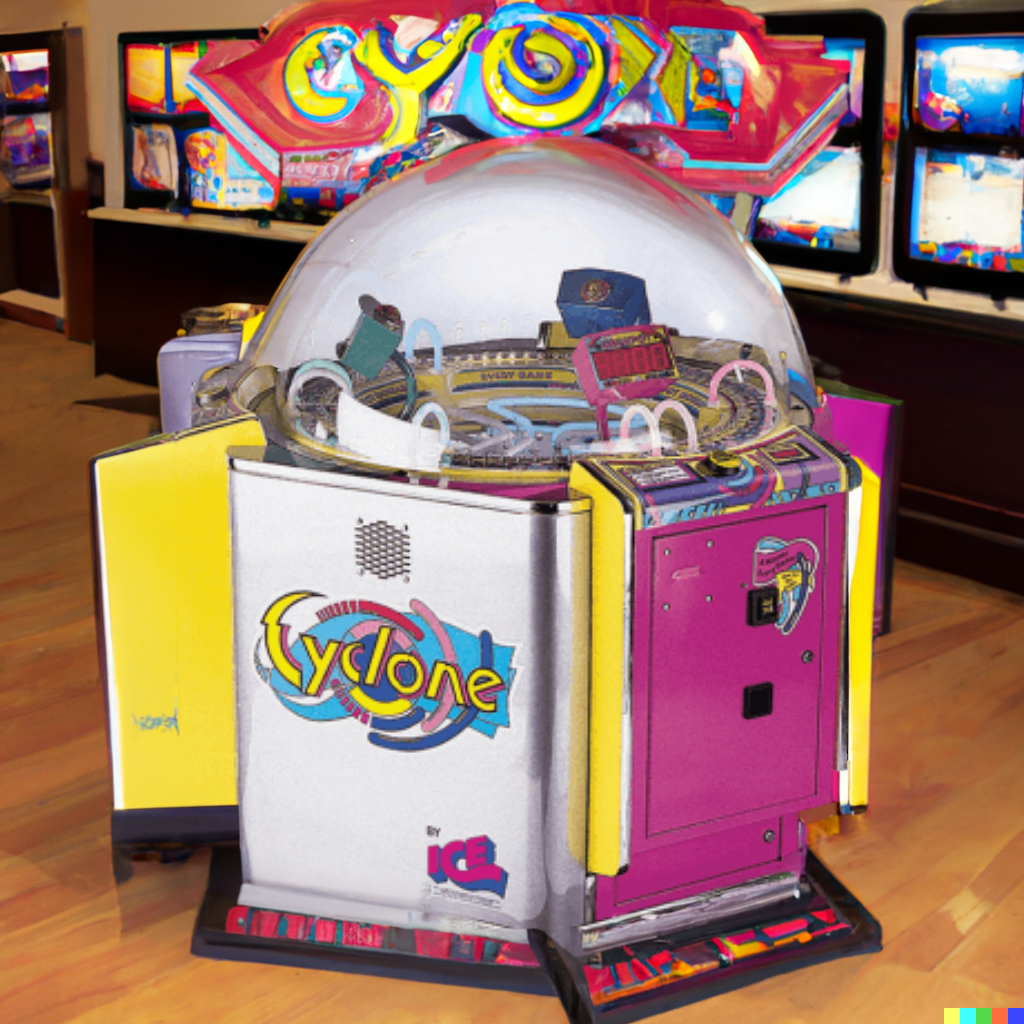
\includegraphics[width = 10cm]{Images/Cyclone (2).png}
    \caption{Cyclone Video Game, from ICE Games edited into location using DALLE2}
    \label{fig:enter-label}
\end{figure}